% 2010 年湖南卷理科第 10 题：⊙O 外一点 P 的切线与割线。
% 来源 PDF：普通高考/2010/2010湖南理.pdf，SHA-256 db6274a80ebb0022ff1b91b2cd3714fe8cca335e48be69805dcd87cdefd8c8d1。
% 原页：第 1 页（A3 三栏）第 2 栏上部，书页码 601。
% 重绘依据：照原页，圆心 O 在圆内偏右上；P 在圆外左下，PT 为切线（T 在圆左上），
%   割线自 P 向右穿过圆于 A（近 P）与 B（远 P），A、B 在圆上，弦 AB 近似水平。
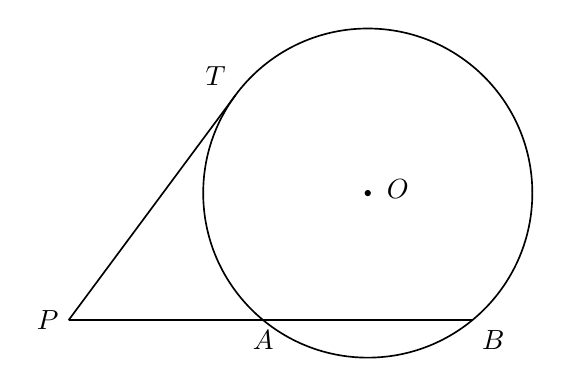
\begin{tikzpicture}[scale=0.95, semithick]
  \coordinate (O) at (0,0);
  \coordinate (P) at (-4,-1.7);
  \coordinate (T) at (-1.767,1.31);
  \coordinate (A) at (-1.396,-1.7);
  \coordinate (B) at (1.396,-1.7);

  \draw (O) circle (2.2);
  \fill (O) circle (1.2pt);
  \node[right] at (0.12,0.06) {$O$};

  \draw (P) -- (T);
  \draw (P) -- (B);

  \node[above left] at (T) {$T$};
  \node[left] at (P) {$P$};
  \node[below] at (A) {$A$};
  \node[below right] at (B) {$B$};
\end{tikzpicture}
